\qns{Statespace Circuit Representation} {\bfseries (Spring 2017 MT 2)}

Consider the circuit below that consists of a capacitor, an
inductor, and a third element with the nonlinear voltage-current characteristic:

$$i = -v + v^3$$

\begin{center}
    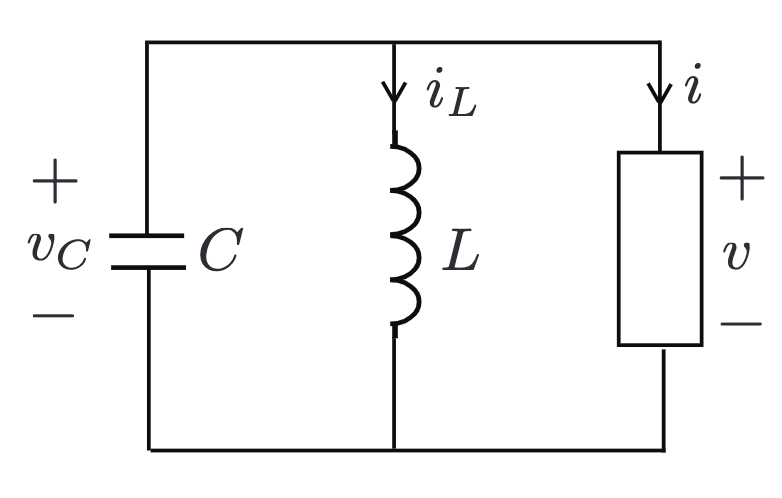
\includegraphics[width = 0.3 \textwidth]{\bank/../fa20/sm-interview/figures/statespace-circuit.png}
\end{center}

\begin{enumerate}
    \qitem Write a statespace model of the form
    \begin{align*}
        \frac{dx_1(t)}{dt} = f_1(x_1(t), x_2(t)) \\
        \frac{dx_2(t)}{dt} = f_2(x_1(t), x_2(t))
    \end{align*}
    using the states $x_1(t) = v_C(t)$ and $x_2(t) = i_L(t)$\\

    \sol{
        Using KCL and KVL at the top node, we have that
        \begin{align*}
            i_C + i_L + i = 0 \\
            v_C = v_L = v
        \end{align*}
        Plugging the voltage-current relation for the capacitor and replacing $v_C$ and $i_L$ with the appropriate state variables:
        \begin{align*}
            C \frac{d v_C(t)}{dt} = -i_L + v - v^3 \\
            \frac{d x_1(t)}{dt} = \frac{1}{C}(x_1(t) - x_1^3(t) - x_2(t))
        \end{align*}
        Now, let's use the current-voltage relation for the inductor to get our second state equation.
        \begin{align*}
            v_L(t) = L\frac{d i_L(t)}{dt} \\
            \frac{dx_2(t)}{dt} = \frac{1}{L} x_1(t)
        \end{align*}
        So, the functions for our statespace model are as follows:
        \begin{align*}
            f_1(x_1, x_2) = \frac{1}{C}(x_1 - x_1^3 - x_2) \\
            f_2(x_1, x_2) = \frac{1}{L} x_1
        \end{align*}
    }

    \qitem Linearize the state model at the equilibrium $x_1^* = x_2^* = 0$ and specify the resulting A matrix. \\
    \sol {
        The $A$ matrix is the Jacobian matrix of the system with respect to $\vec{x} = \begin{bmatrix} x_1 & x_2 \end{bmatrix}^T$.
        \begin{align*}
            A = \begin{bmatrix}
                \frac{\partial f_1}{x_1} \bigg\rvert_{x_1^*, x_2^*} & \frac{\partial f_1}{x_2} \bigg\rvert_{x_1^*, x_2^*} \\
                \frac{\partial f_2}{x_1} \bigg\rvert_{x_1^*, x_2^*} & \frac{\partial f_2}{x_2} \bigg\rvert_{x_1^*, x_2^*}
            \end{bmatrix} \\
            A = \begin{bmatrix}
                \frac{1}{C}(1 - 3(x_1^*)^2) & -\frac{1}{C} \\
                \frac{1}{L} & 0
            \end{bmatrix} = \begin{bmatrix}
                \frac{1}{C} & -\frac{1}{C} \\
                \frac{1}{L} & 0
            \end{bmatrix}
        \end{align*}
    }

    \qitem Determine stability based on the linearization. \\
    \sol {
        To determine whether the system is stable, find the eigenvalues by setting the determinant of $A - \lambda I$ to 0:
        \begin{align*}
            -\lambda(\frac{1}{C} - \lambda) + \frac{1}{LC} = 0 \\
            \lambda^2 - \frac{1}{C} \lambda + \frac{1}{LC} = 0 \\
            \lambda = \frac{1}{2C} \pm \frac{1}{2} \sqrt{\frac{1}{C^2} - \frac{4}{LC}}
        \end{align*}
        As you can see, the eigenvalues are positive, so the system is unstable.
    }


\end{enumerate}